En el capítulo Estado del Arte para Proyecto de Titulación \cite{Gonzalez2020EstadoTitulacion} se compararon tres sistemas diferentes para la implementación de adquisición de datos para física de partículas. En ellos destacan aspectos comunes de implementación: etapas de detección de eventos, memorias para almacenamiento temporal, procesamiento de los datos y la utilización de FPGA como herramienta principal para la implementación del hardware.



\section{Alternativas de Solución}
\subsection*{Esquema General}
Tal como se ha planteado en informes anteriores, el esquema básico a implementar es el indicado en la figura \ref{fig:diagrama}. Se requieren al menos tres etapas esenciales: discriminar, procesar y analizar. Discriminar se refiere a distinguir entre aquellos eventos que corresponden un muón de aquellos que no, descartando estos últimos. Procesar implica utilizar los pulsos escogidos, formar una estructura que los relacione como un solo evento y posiblemente incluir información de ellos, como una marca temporal y la duración de los pulsos captados en dicho evento. 

La etapa de análisis implica mayor complejidad y puede extenderse para abarcar distintos niveles. El análisis más básico implica leer un evento e inferir la región del detector que fue excitada por el paso del muón. Niveles siguientes implicarían estimar la energía del muón, incluir mayor precisión espacial, correlacionar con eventos anteriores o incluso trazar la trayectoria  del paso de la partícula al superponer los datos de eventos originados en otros detectores.

\newpage
\subsection*{Requisitos}
Las alternativas aquí propuestas deberán cumplir con las especificaciones mínimas necesarias para captar los pulsos digitales provenientes del detector de muones. Estos requisitos son los siguientes:

\begin{itemize}
	\item Se debe contar con al menos 32 pares de entradas bajo el estándar LVDS, con el fin de conectar al menos 2 tarjetas ASD (Amplificator Shaper Discriminator) utilizadas cada una como la interfaz de detectores de 16 canales.
	\item Es importante contar con un reloj presente o sintetizable de una frecuencia mayor a 100[MHz], lo más cercano a 1[GHz] posible, con el fin de captar la duración de los pulsos y el momento de aparición de un evento con la mayor precisión disponible.
	\item Se debe considerar que la señal de disparo que entrará al sistema estará desfasada cerca de 100[ns] respecto al paso real de los muones por el detector, siendo necesaria la implementación de delays para las señales capturadas o un sistema capaz de distinguir la ocurrencia de eventos y disparos en el tiempo.
	\item  Se debe tener la capacidad de mantener señales sincronizadas, guardar información en memorias temporales y llevar cuenta del transcurso del tiempo entre eventos.
	\item Es requisito que la implementación de la alternativa permita escalamiento para agregar nuevos detectores adyacentes con el fin de aumentar el área de prueba, así como también sincronizarse con detectores paralelos para trazar trayectorias de las partículas captadas.
\end{itemize}

En cuanto a los requisitos de tiempo y reloj de operación anteriormente indicados, estos se deben esencialmente a que la duración de un pulso digital proveniente de un detector podría estar entre 1[ns] y 40[ns]\cite{1999ATLASICs}. Este ancho de pulso tiene correlación con la amplitud del pulso análogo original y el error en su medición implicará menor precisión en la estimación de esta variable.

Respecto a la tasa de aparición de pulsos consecutivos, es poco probable que ocurran eventos simultáneos o cercanos. Se espera que la tasa de muones por centímetro cuadrado sea de un muón por minuto, lo que en los $15[cm^2]$ representados por una señal de detector implicaría cerca de 15 muones por minuto o $2,5*10^{10}$ muones cada 100 [ns], lo que se traduce a una muy baja probabilidad de eventos simultáneos o incluso cercanos. De hecho, la tasa de detección de muones puede disminuir estando bajo tierra y se planea que la toma de una muongrafía conlleve un tiempo prolongado de exposición a rayos cósmicos. Esto conduce a la conclusión de que ignorar posibles eventos simultáneos o adyacentes no tendrá implicancias significativas en los resultados de la muongrafía final.

%\par Dicho lo anterior y planteadas las bases para el desarrollo de alternativas, se presentan a continuación 4 opciones para desarrollar el proyecto de titulación "Sistema de Adquisición de Datos para Detectores de Muones".
%
%
%\newpage
%\subsection{Digitizer}
%Como primera alternativa, se propone la utilización de Digitizers. Estos aparatos son equipos digitalizadores de múltiples canales que permiten guardar en un computador la información de los pulsos captados.
%\par El laboratorio en el cual se desarrolla este proyecto cuenta con digitalizadores CAEN modelo DT5730 (8 canales, 500[MS/s] y 2Vpp de rango de entrada) y modelo DT5740 (32 canales, 62,5[MS/s] y 2Vpp de rango de entrada). 
%\par De los dos equipos considerados, es razonable utilizar el DT5740. Este es capaz de leer al menos 32 canales, suficiente para trabajar con dos detectores de 16 señales. Dada su baja tasa de muestreo, se dificulta la opción de cuantificar el ancho de los pulsos captados, por lo que solo sería fiable la detección posición de muones. Aún así, podría existir error en la sincronización del disparo respecto a los pulsos captados en máximo 17[ns] debido a la baja tasa de muestreo.
%
%\par Adicionalmente a la utilización del equipo digitalizador, se hace necesaria la confección de una interfaz que adapte las señales de tipo LVDS provenientes del acondicionador de señales (ASD) hacia un voltaje legible por el digitizer, el cual podría ser en standard TTL 3.3[V] o CMOS. Tendrá que incluir también lineas o circuitos integrados de retardo para cada una de las señales captadas, del orden de 100[ns] para ser sincrónica con la señal de disparo. La salida de esta nueva tarjeta tendrá que conectarse al digitalizador con cable coaxial de $50[\Omega]$, idealmente de conector LEMO a conector MCX, existentes en el laboratorio y exigido por el digitalizador. La interconexión de esta placa con el resto de los equipos se ilustra en la figura \ref{fig:digitizer1}.
%
%\begin{figure}[H]
%	\centering
%	\includegraphics[scale=1]{imagenes/digitizer1.pdf}
%	\caption{Diagrama de conexiones utilizando un digitalizador CAEN DT7540 y un solo detector de muones. La señal de disparo se encuentra disponible en formato LVDS y TTL.}
%	\label{fig:digitizer1}
%\end{figure}
%
%
%\par Lo descrito anteriormente correspondería a la etapa de captura y discriminación. Para la etapa de procesamiento será necesaria la utilización de software programado en un computador para generar estructuras de datos con información pertinente para el análisis y luego para la implementación del análisis de los eventos captados. La estructura base para este software se ilustra en la figura \ref{fig:digitizer2}
%
%\begin{figure}[H]
%	\centering
%	\includegraphics[scale=1]{imagenes/digitizer2.pdf}
%	\caption{Diagrama de bloques del software, utilizando un digitalizador CAEN DT7540. El módulo de control se encuentra implementado y disponible, basado en librerías del fabricante. Las entradas y salidas de estos bloques son arreglos de datos relacionando la señal con su información. Para el manejo de estos datos se utiliza el framework ROOT\cite{CERN2020ROOT:Framework}. El bloque de formateo ajusta la estructura de datos original para facilitar el procesamiento. El bloque de procesamiento lee los datos determinando el ancho de ellos y asociandolo al canal correspondiente. El bloque de análisis se encarga de estimar la coordenada y eventualmente la energía asociada a cada evento.}
%	\label{fig:digitizer2}
%\end{figure}
%
%
%\par El sistema actualmente descrito es muy similar al procedimiento y configuración circuital utilizados para estudios previos a este proyecto. Se han realizado pruebas al detector en crudo con señales analógicas captadas por digitalizadores de pocos canales, procesando y analizando posteriormente los pulsos para comprobar calidad y factibilidad.
%
%\subsubsection*{Atributos}
%\begin{itemize}
%	\item \textbf{Simplicidad:} Media. Requiere la fabricación de una PCB de interfaz y la integración de 3 aparatos distintos (Digitalizador, interfaz y computador).
%	\item \textbf{Desempeño:} Bajo. Baja tasa de muestreo.
%	\item \textbf{Disponibilidad:} Media. Se cuenta con un digitalizador, pero no está disponible una interfaz LVDS a TTL.
%	\item \textbf{Economía:} Baja. El costo de digitalizadores adicionales podría superar los US\$1000.
%\end{itemize}
%
%\subsubsection*{Ventajas}
%\begin{itemize}
%	\item Planificación simplificada.
%	\item Etapas claras.
%	\item Adaptable en etapa de software.
%\end{itemize}
%
%
%\subsubsection*{Desventajas}
%\begin{itemize}
%	\item Baja tasa de muestreo.
%	\item Alto costo.
%	\item Poco práctico.
%	\item Difícil escalamiento.
%	\item Requiere fabricación de hardware adicional.
%\end{itemize}

%\newpage
%\subsection{Microcontrolador}
%\label{sec:micro}
%\par Una alternativa común en el rubro de la electrónica es el uso de microcontroladores. Destacan por su versatilidad pero no son aplicables a todos los casos. Para esta alternativa de solución se buscaron placas de desarrollo con microcontroladores con un número de entradas y frecuencia de reloj razonable, pero no fue posible encontrar uno que cumpliera con todo lo necesario. 
%\par En afán de utilizar un microcontrolador como alternativa comparativa, se plantea la posibilidad de utilizar múltiples unidades de manera paralela, logrando satisfacer el requisito de cantidad de señales.
%
%\par Dado que se requiere trabajar con señales LVDS, se vuelve necesario incluir conversores LVDS-TTL en esta alternativa de solución. Para captarlas y medirlas sería necesaria la existencias de conversores análogo-digitales (ADC) para muestrear las señales. Si bien son originalmente de naturaleza digital, no es posible captarlas y muestrearlas con facilidad sin la utilización de ADCs.
%
%\par Para trabajar con la señal de disparo desfasada, se pueden utilizar memorias incluidas en las placas de desarrollo para almacenar los pulsos en orden de llegada mientras se espera por una señal de disparo. En el momento de su llegada, es posible buscar en memoria los pulsos que hayan sido muestreados en un tiempo atrás equivalente al desfase del disparo y estructurar la información como un nuevo evento válido.
%
%\par Dada la baja frecuencia de reloj que se encuentra comúnmente en las tarjetas de desarrollo de microcontroladores, se dificulta la operación y precisión del sistema. Si bien esto puede mejorar con la frecuencia de muestreo de los ADC, sigue siendo difícil y costoso acercarse a 1[]GSPS].
%
%\par Finalmente, las etapas de procesamiento se pueden ver facilitadas en esta alternativa. La implementación de ellas en un microcontrolador suele ser más intuitiva y óptima dada su naturaleza para trabajar operaciones matemáticas. Por otro lado, sincronizar los eventos y los datos entre microcontroladores adyacentes puede ser un desafío considerable. En las figuras \ref{fig:microcontrolador1}, \ref{fig:microcontrolador2}, y \ref{fig:microcontrolador3} se ilustra esta propuesta en base a un microcontrolador.
%
%\begin{figure}[H]
%	\centering
%	\includegraphics[scale=1]{imagenes/microcontrolador1.pdf}
%	\caption{Diagrama de bloques utilizando microcontroladores como alternativa de solución con un solo detector. Dado que el numero de puertos es bajo, puede ser necesario utilizar dos microcontroladores por cada detector. Además, se hace necesario un microcontrolador adicional para captar y relacionar los eventos de las etapas anteriores, unificándolos en un solo evento.}
%	\label{fig:microcontrolador1}
%\end{figure}
%
%\begin{figure}[H]
%	\centering
%	\includegraphics[scale=1]{imagenes/microcontrolador2.pdf}
%	\caption{Representación en diagramas de bloques de los elementos internos de uno de los microcontroladores iniciales. Se encarga de captar la mitad de los pulsos originados por un detector. El bloque ADC muestrea los pulso en el tiempo, almacenándolos en una cola de datos FIFO. Un controlador de esta cola determina el avance o descarte de datos en función de las señales de disparo captadas. El bloque sincronizador apoya la operación de dos microcontroladores simultáneos, asegurándose que ambos capten los mismos eventos. El estructurador de datos da forma a la información, asociando duración de pulso a cada uno de los canales captados, para luego enviarlo a la siguiente etapa mediante comunicación serial.}
%	\label{fig:microcontrolador2}
%\end{figure}
%
%\begin{figure}[H]
%	\centering
%	\includegraphics[scale=1]{imagenes/microcontrolador3.pdf}
%	\caption{Representación en diagramas de bloques de los elementos internos del microcontrolador final. Se encarga de unificar eventos de dos microcontroladores distintos, incluso pudiendo escalarse a unificar eventos procedentes de más detectores. Aquí existe un segundo bloque estructurador, encargado de unificar, entregando una estructura de igual notación pero mayor tamaño. El bloque de análisis de coordenadas permite la estimación de la coordenada por la cual ha pasado la partícula y eventualmente la energía asociada, para luego enviar esta información a una etapa siguiente de análisis profundo mediante comunicación serial.}
%	\label{fig:microcontrolador3}
%\end{figure}
%
%
%\newpage
%\subsubsection*{Atributos}
%\begin{itemize}
%	\item \textbf{Simplicidad: } Baja. Gran cantidad de dispositivos.
%	\item \textbf{Desempeño: } Bajo. Bajas tasas de muestreo y operación.
%	\item \textbf{Disponibilidad: } Baja. Todos los materiales tendrían que ser adquiridos.
%	\item \textbf{Economía: } Baja, poco económico. Si bien las tarjetas de desarrollo pueden ser de bajo costo, se necesitan varias y se agregan componentes extra que aumentan el costo considerablemente.
%\end{itemize}
%
%\subsubsection*{Ventajas}
%\begin{itemize}
%	\item Escalable.
%	\item Tecnologías muy conocidas.
%	\item Facilita el análisis y operaciones matemáticas.
%\end{itemize}
%
%
%\subsubsection*{Desventajas}
%\begin{itemize}
%	\item Costoso.
%	\item Bajo desempeño.
%	\item Varias fuentes de error, dada su complejidad.
%	\item Poca disponibilidad de los materiales y hardware necesario.
%\end{itemize}

%\newpage
%\subsection{CPLD}
%\par Otra alternativa de solución consiste en describir módulos de hardware en una CPLD (Complex Programable Logic Device). Estos dispositivos tienen la ventaja de ser de bajo costo, pero con la condición de contar con pocos recursos lógicos para su operación.
%\par Contar con la posibilidad de describir el hardware en su interior facilita la implementación del sistema, logrando resultados mejor adaptados al problema real.
%\par Una tarjeta de desarrollo para CPLD es la Lattice MACH X02\cite{Semiconductor2017DS1035Sheet}. Esta tarjeta cuenta con cerca de 7000 LUTs (Look-up tables), cerca de 250kb de memoria RAM, relojes sintetizables de hasta 400MHz y particularmente 114 puertos LVDS, suficientes para conectar al menos dos detectores sin tarjetas intermedias con hardware adicional. Esto no quita que se requiera de una tarjeta o adaptador para conectar las señales del detector a la tarjeta de desarrollo.
%
%\par Las grandes desventajas de esta tarjeta son sus escasos recursos disponibles y nulos periféricos. Si bien sus frecuencias de reloj son destacables, aún pueden ser mejores en otras alternativas.
%
%\par La implementación propuesta para esta alternativa rescata elementos de alternativas anteriores, en especial para el tratamiento del desfase de la señal de disparo, rescatando eventos anteriormente guardados en memoria. Su mayor frecuencia de reloj permite el tratamiento de las señales con una precisión mayor y más razonable, teniendo errores de cerca de 2.5[ns] en el arribo de señales y en la medición de anchos de pulso. Las figuras \ref{fig:cpld1}, \ref{fig:cpld2}, \ref{fig:cpld3} reflejan la solución propuesta.
%
%\par Para la etapa de análisis se hace necesario el apoyo de un computador que tome los paquetes de eventos procesados por la CPLD y sea capaz de extraer la información de interés.
%
%\begin{figure}[H]
%	\centering
%	\includegraphics[scale=1]{imagenes/cpld1}
%	\caption{Diagrama de bloques utilizando una CPLD como alternativa de solución.}
%	\label{fig:cpld1}
%\end{figure}
%
%
%
%\begin{figure}[H]
%	\centering
%	\includegraphics[scale=1]{imagenes/cpld2}
%	\caption{Diagrama de bloques de la lógica interna descrita para la CPLD. Similar a la estructura interna propuesta para los microcontroladores iniciales de la figura \ref{fig:microcontrolador2}. Aquí no existe sincronización explicita con una segunda CPLD ya que solo se utiliza una por detector. El estructurador de datos cumple la misma función de asociar duración de pulso a cada canal medido del evento. Las etapas de análisis no se realizan y se delegan a una etapa posterior.}
%	\label{fig:cpld2}
%\end{figure}
%
%\newpage
%\begin{figure}[H]
%	\centering
%	\includegraphics[scale=1]{imagenes/cpld3}
%	\caption{Representación del software presente en un computador de apoyo. Su estructura y funcionamiento cumple la misma idea de lo planteado para la primera alternativa de solución, como ilustra la figura \ref{fig:digitizer2}.}
%	\label{fig:cpld3}
%\end{figure}
%
%
%\par En cuanto al escalamiento, sería factible utilizar una CPLD cada dos detectores. Aún así, se debería tener la precaución de optimizar el hardware a un nivel tal que los recursos sean suficientes para la implementación.
%
%\subsubsection*{Atributos}
%\begin{itemize}
%	\item \textbf{Simplicidad:  } Alta. Pocos dispositivos involucrados.
%	\item \textbf{Desempeño:}  Medio. Escasos recursos lógicos y periféricos.
%	\item \textbf{Disponibilidad:}  Alta. Se cuenta con una de estas tarjetas en el laboratorio.
%	\item \textbf{Economía: } Alta. Una de estas tarjetas tiene un valor cercano a los US\$30.
%\end{itemize}
%
%\subsubsection*{Ventajas}
%\begin{itemize}
%	\item Muy económica.
%	\item Alta frecuencia de reloj comparada con alternativas anteriores.
%	\item Cuenta con puertos LVDS.
%	\item Escalable.
%\end{itemize}
%
%
%\subsubsection*{Desventajas}
%\begin{itemize}
%	\item Pocos recursos lógicos disponibles.
%	\item Escasa memoria para almacenar pulsos y eventos
%	\item Pocos periféricos, prácticamente solo cuenta con comunicación serial.
%	\item Se requiere confeccionar un adaptador para conectar el detector con la tarjeta de desarrollo.
%\end{itemize}

\newpage
\subsection{FPGA}
La alternativa más utilizada en el rubro es la FPGA. Esta ha sido la herramienta que se ha visto con mayor frecuencia en proyectos relativos a física de partículas y adquisición de datos. 
Las FPGA cuentan con una cantidad significativa de recursos y periféricos. Incluyen además hardware dedicado para comunicación, serialización y almacenamiento de datos. Incluso suelen incluir CPLDs en las placas que las albergan. Una desventaja conocida corresponde a que se basan en memorias volátiles, por lo que el hardware descrito se debe reconfigurar cada vez que se enciende, y los datos importantes deben ser almacenados en memorias externas.

Para esta alternativa se propone el uso de la tarjeta de desarrollo Trenz TR0712 \cite{TrenzElectronic2019TR07012Wiki} montada en una placa TR0703 \cite{TrenzElectronic2019TR0703Wiki}. Esta tarjeta en su conjunto se basa en una FPGA Xilinx Artix 7 \cite{Xilinx20107DS180} de cerca de 16.000 celdas lógicas, incluyendo además chips de memoria RAM, reloj de 20[MHz] con hasta 600[MHz] sintetizables, comunicación Ethernet y por supuesto puertos LVDS suficientes para conectar al menos 2 detectores.

Si bien esta tarjeta cuenta con puertos LVDS, será necesario confeccionar un adaptador para conectar las señales del detector hacia la placa Trenz.

%En esta alternativa se rescatan los diseños de hardware mencionados con anterioridad, con la holgura de que existen recursos suficientes para implementar los bloques indicados. Incluso se evalúa incluir parte del análisis dentro de la FPGA y no destinarla a un computador en su totalidad.

La frecuencia de reloj que puede alcanzar esta tarjeta es mucho mayor que cualquiera de las anteriores, siendo entonces la que permite tener mayor precisión en términos de tiempo, sobretodo para determinar la duración de los pulsos provenientes del detector.

La idea en esta alternativa de solución es guardar los datos en memoria temporal hasta la llegada de una señal de disparo. Un módulo que maneja la memoria será el encargado de tomar los pulsos correspondientes al disparo recibido y liberar la memoria de aquellos datos ya leídos u obsoletos, entregando la información útil a una siguiente etapa. Los pulsos aceptados serán entonces relacionados como parte de un mismo eventos y se estimará la duración de estos, generando y guardando así un arreglo de datos con identificador de pulso y duración. La última etapa se encargará de efectuar una operación capaz de determinar la posición del evento a partir de las duraciones medidas y los pulsos detectados, comunicando así un arreglo básico y preprocesado que incluya posición y magnitud aproximada.

\par Se espera que para lograr el escalamiento se incluya una señal para mantener la lectura de eventos sincronizada entre distintas FPGA. Además, se deberá incluir un modulo de comunicación para entregar la información captada a una etapa posterior con un análisis más detallado, encargado de reunir todos los eventos de diferentes FPGAs.

\newpage
\par Las figuras \ref{fig:fpga1} \ref{fig:fpga2} ilustran conexiones y bloques a implementar en esta alternativa de solución.

\begin{figure}[H]
	\centering
	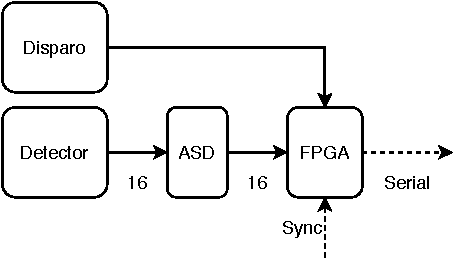
\includegraphics[scale=1]{imagenes/fpga1.pdf}
	\caption{Diagrama de bloques utilizando una FPGA como alternativa de solución. Se indica una salida serial para transmitir los resultados del análisis básico a algún procesador o memoria de alguna etapa posterior. La señal de sincronización, inspirada en la alternativa \ref{sec:micro} tiene como objetivo sincronizar la recolección y procesamiento de eventos, para que estos sean consistentes entre detectores.}
	\label{fig:fpga1}
\end{figure}

\begin{figure}[H]
	\centering
	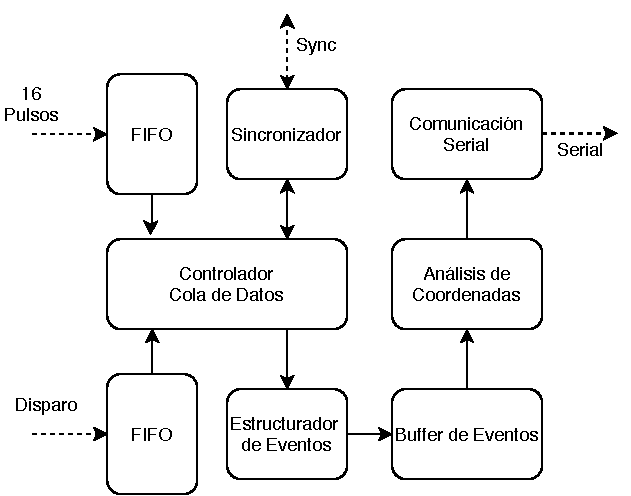
\includegraphics[scale=1]{imagenes/fpga2.pdf}
	\caption{Representación de la lógica interna de la FPGA. Se agrega una cola de datos para las señales de disparo y una memoria de almacenamiento temporal para los eventos ya estructurados. Ambas implementaciones permiten tener mejor control del flujo de datos, evitando perdidas y asegurando sincronía a pesar de que la lectura de la información sea eventualmente más lenta que la captura de pulsos. Los bloques controlador, estructurador y análisis cumplen las mismas funciones mencionadas en alternativas anteriores: aceptar o descartar pulsos, cuantificar anchos de pulso a  los canales asociados y determinar coordenada del cruce de un muón respectivamente.}
	\label{fig:fpga2}
\end{figure}

\newpage
\subsubsection*{Atributos}
\begin{itemize}
	\item \textbf{Simplicidad:}  Media. Gran cantidad del sistema concentrado en una sola placa, pero aumenta la dificultad en la descripción de hardware.
	\item \textbf{Desempeño:}  Alto. Gran cantidad de recursos lógicos, de almacenaiento y de frecuencia de operación.
	\item \textbf{Disponibilidad: } Alta. Se cuenta con una en el laboratorio.
	\item \textbf{Economía: } Media. Una tarjeta de desarrollo de este estilo tiene un costo de aproximadamente US\$400.
\end{itemize}

\subsubsection*{Ventajas}
\begin{itemize}
	\item Gran cantidad del sistema concentrado en una sola placa.
	\item Escalable
	\item Cuenta con puertos LVDS
	\item Alta densidad de recursos lógicos
	\item Dispone de memoria suficiente para almacenar eventos
	\item Posee una alta frecuencia de reloj sintetizable, mejorando precisión temporal.
	\item Placa con muy buena documentación.
\end{itemize}


\subsubsection*{Desventajas}
\begin{itemize}
	\item Se requiere confeccionar un adaptador para conectar el detector con la tarjeta de desarrollo.
	\item Se complica el diseño y la implementación del hardware.
\end{itemize}




%\newpage
%\section{Conclusiones}
%\par Luego de estudiar cuatro alternativas de solución, es posible aseverar que una FPGA cuenta con la mayor capacidad para cumplir con los objetivos de este proyecto.
%\par Si bien otras alternativas pueden tener ventajas en cuanto a precio, una FPGA simplifica algunas labores y da la holgura necesaria para implementar el sistema descrito.
%\par Una quinta alternativa muy interesante es la utilización de una FPGA en conjunto con un procesador, como es el caso de las Zynq, mencionadas en informes anteriores. Estos dispositivos no fueron considerados ya que en el laboratorio no se encuentran disponibles tarjetas de desarrollo que cumplan con las especificaciones planteadas, particularmente con el número de puertos LVDS accesibles y necesarios para la confección del detector.
%\par Otra alternativa descartada ha sido la aplicación de TDC (Time to Digital Converter)\cite{Arpin2010AResources}, que si bien permitiría mejorar la resolución temporal del sistema, implica un desafío ingenieril y de recursos a una escala un tanto mayor.
%\par Estas dos últimas propuestas quedan disponibles para ser implementadas en iteraciones posteriores, una vez que se tenga certeza del funcionamiento básico requerido que el actual proyecto plantea.


%%%%%%%%%%%%%%%%%%%%%%%%%%%%%

¿Cuáles son las etapas esenciales que un DAQ debe poseer? En esencia se requiere de una primera etapa de interfaz de lectura directamente de los detectores (\textit{Readout}), las cuales suelen poseer amplificadores, modeladores de pulsos, memorias y digitalizadores. Una segunda etapa suele consistir en el preprocesamiento de las señales, extrayendo la información básica y formando estructuras de datos pertinentes. Finalmente, está la etapa de procesamiento fuera del detector, donde se realiza el análisis e interpretación de los datos.

En este proyecto de titulación, la primera etapa la lleva a cabo la tarjeta acondicionadora ASD (Amplifier Shaper Discriminator), diseñada para detectores del proyecto ATLAS. Las etapas restantes serán diseñadas pensando en la aplicación específica de este proyecto.

%En el documento ``Alternativas de Solución de Proyecto de Titulación'' se presentaron 4 posibles alternativas para la implementación de un sistema de adquisición de datos para detectores de muones. En cada una de ellas se proponen distintas tecnologías para llevar acabo el mismo fin: Digitizers, Microcontroladores, CPLDs y FPGAs. La figura \ref{fig:diagrama} ilustra la estructura general del sistema de adquisicón de datos.
%
%En el actual documento se presenta el contraste entre las 4 alternativas discutidas con anterioridad, asignando puntaciones a cada una de ellas en base a criterios clave asociados a las características y el diseño del sistema. Los criterios a evaluar son: simplicidad, desempeño, disponibilidad, economía, flexibilidad y documentación. La comparativa que se desarrolla aquí tiene como objetivo definir cuál de las 4 opciones es la mejor alternativa a desarrollar, cumpliendo además con los requisitos principales del proyecto.
%
%La alternativa seleccionada se presenta y detalla a continuación de la comparación de alternativas, planteando sus características principales y justificando la elección realizada.
%\begin{figure}[H]
%    \centering
%    
%    \tikzstyle{externo} = [rectangle, rounded corners, minimum width=2cm, minimum height=1cm,text centered, draw=black, fill=blue!30]
%    \tikzstyle{fpga} = [rectangle, rounded corners, minimum width=3cm, minimum height=2.5cm,text centered, draw=black, fill=green!30]
%    \tikzstyle{flecha} = [thick,->,>=stealth]   
%    
%    \begin{tikzpicture}[node distance=1.5cm]
%
%        \node (disparo) [externo] {Disparo};
%        \node (detector) [externo, below of=disparo] {Detector};
%        \node (asd) [externo, right of=detector, xshift=1cm] {ASD};
%        \node (disc) [fpga, right of=detector, xshift=2.5cm, yshift=-0.5cm, anchor=south west] {Discriminador};
%        \node (pros) [fpga, right of=disc, xshift=2cm] {Procesamiento};
%        \node (res) [fpga, right of=pros, xshift=2cm] {Análisis};
%        
%        \draw [flecha] (disparo) --  (disc.west |- disparo);
%        \draw [flecha] (detector) -- (asd);
%        \draw [flecha] (asd) -- (disc.west |- asd);
%        \draw [flecha] (disc) -- (pros);
%        \draw [flecha] (pros) -- (res);
%
%    \end{tikzpicture}
%
%    \caption{Diagrama de bloques del sistema. En azul se presentan las etapas previas al proyecto que ya se encuentran desarrolladas y sobre las cuales no se tiene control. En verde se ilustran las etapas pendientes y que pueden ser desarrolladas en este proyecto. El disparo corresponde a la señal digital que indica si la partícula detectada es un muón y el ASD es un acondicionador de señal que genera pulsos digitales a partir de los pulsos analógicos captados.}
%    \label{fig:diagrama}
%\end{figure}


%\section{Criterios de Selección}
%\par Para seleccionar la alternativa más adecuada se definieron seis distintos criterios de evaluación, cada uno de los cuales puede obtener un puntaje entre 1 y 10. Los criterios tienen distinta relevancia dentro del proyecto, resultando en que algunos de ellos tengan mayor ponderación respecto a otros. La tabla \ref{tab:criterios} indica el porcentaje de relevancia correspondiente cada criterio de selección. 
%
%\begin{table}[H]
%	\centering
%	\begin{tabular}{|l|c|}
%		\hline
%		\textbf{Criterio de Selección} & \textbf{Porcentaje de Relevancia} \\ \hline
%		Simplicidad & 10\% \\ \hline
%		Desempeño & 35\% \\ \hline
%		Disponibilidad & 25\% \\ \hline
%		Economía & 10\% \\ \hline
%		Flexibilidad & 10\% \\ \hline
%		Documentación & 10\% \\ \hline
%		\textit{Total} & \textit{100\%} \\ \hline
%	\end{tabular}
%	\caption{Porcentaje de relevancia para cada criterio.}
%	\label{tab:criterios}
%\end{table}
%
%\newpage
%\par Se considera como criterio de mayor importancia al \textit{desempeño} estimado de la alternativa, ya que será el aspecto que defina la calidad y funcionamiento del sistema. En segundo lugar de relevancia se ubica la \textit{disponibilidad} de recursos, ya que sin ellos no es posible construir el dispositivo. Los criterios restantes se consideraron menor con ponderación ya que son importantes, pero no cruciales para llevar a cabo el proyecto en su primera versión.
%\par Cada criterio es evaluado con un puntaje de 1 a 10 puntos en una escala indicada en la tabla \ref{tab:escala}. A continuación se detalla cada criterio, incluyendo su descripción y explicando la interpretación de puntaje según la escala mencionada.
%
%\begin{table}[H]
%	\centering
%	\begin{tabular}{lllll}
%		\hline
%		\multicolumn{1}{|c|}{\textbf{Muy Baja}} & \multicolumn{1}{c|}{\textbf{Baja}} & \multicolumn{1}{c|}{\textbf{Media}} & \multicolumn{1}{c|}{\textbf{Alta}} & \multicolumn{1}{c|}{\textbf{Muy Alta}} \\ \hline
%		\multicolumn{1}{|c|}{1 - 2}                 & \multicolumn{1}{c|}{3 - 4}             & \multicolumn{1}{c|}{5 - 6}           & \multicolumn{1}{c|}{7 - 8}           & \multicolumn{1}{c|}{9 - 10}              \\ \hline 
%	\end{tabular}
%	\caption{Tabla de puntajes para criterios de evaluación.}
%	\label{tab:escala}
%\end{table}
%
%\subsection*{Simplicidad}
%\par El criterio de simplicidad se refiere a la dificultad de diseñar, programar, fabricar y ensamblar el sistema descrito en la alternativa evaluada. La máxima simplicidad está indicada con un puntaje 10 y la mínima simplicidad con un puntaje 1. Máxima simplicidad implica conectar elementos sin mayor esfuerzo, prácticamente no programar software y prácticamente no diseñar ni implementar hardware. Mínima simplicidad implicaría dificultad de interconexión entre elementos componentes, debido a sus estándares o cantidad de conexiones presentes, incluyendo software de alta complejidad y prácticamente el desarrollo completo del hardware.
%
%\subsection*{Desempeño}
%La evaluación por desempeño tiene directa relación con los requisitos de diseño asociados al sistema a desarrollar. Estos requisitos son los siguientes:
%
%\begin{itemize}
%	\item Se debe contar con al menos 32 pares de entradas bajo el estándar LVDS, con el fin de conectar al menos 2 tarjetas ASD (Amplificator Shaper Discriminator) utilizadas cada una como la interfaz de detectores de 16 canales.
%	\item Es importante contar con un reloj presente o sintetizable de una frecuencia mayor a 100[MHz], lo más cercano a 1[GHz] posible, con el fin de captar la duración de los pulsos y el momento de aparición de un evento con la mayor precisión disponible.
%	\item Se debe considerar que la señal de disparo que entrará al sistema estará desfasada cerca de 100[ns] respecto al paso real de los muones por el detector, siendo necesaria la implementación de retardos para las señales capturadas o un sistema capaz de distinguir la ocurrencia de eventos y disparos en el tiempo.
%	\item  Se debe tener la capacidad de mantener señales sincronizadas, guardar información en memorias temporales y llevar cuenta del transcurso del tiempo entre eventos.
%	\item Es requisito que la implementación de la alternativa permita escalamiento para agregar nuevos detectores adyacentes con el fin de aumentar el área de prueba, así como también sincronizarse con detectores paralelos para trazar trayectorias de las partículas captadas.
%\end{itemize}
%
%\par Sintetizando estos requisitos, es posible acotarlos a  5 elementos esenciales: número de canales, disponibilidad de puertos LVDS, frecuencia de reloj, implementación o manejo de retardos y recursos de almacenamientos o procesamiento disponibles. La escalabilidad queda implícitamente evaluada con los criterios de simplicidad, economía y flexibilidad.
%
%\par Considerando lo anterior, se le asignará puntaje a este criterio en función de la cantidad de requisitos que cumpla y la calidad con la que sean satisfechos, considerando 10 puntos en caso de cumplir a cabalidad con todos ellos, y asignándole 1 punto en caso de cumplir ninguno.
%
%\subsection*{Disponibilidad}
%\par El criterio de disponibilidad evalúa la presencia inmediata de los materiales necesarios para la implementación del sistema. Pondera la cantidad de elementos necesarios como un total de 10 puntos repartidos en cada uno de los elementos componentes para construir un sistema de adquisición de 32 canales. Si un sistema requiere de 5 elementos discretos, tendrá entonces 10 puntos en caso de contar con la disponibilidad de los 5 elementos necesarios. Si alguno no está disponible y requiere ser adquirido, entonces implicaría un descuento de 2 puntos en dicho ejemplo.
%
%\subsection*{Economía}
%\par El criterio de economía evalúa el precio total de construcción del dispositivo, incluyendo todo el hardware necesario para la discriminación, procesamiento y análisis, sin considerar un computador en las etapas finales de análisis o recolección de información. Este criterio es útil para contrastar la factibilidad de escalamiento. Un sistema muy costoso implicará dificultades para replicarlo.
%\par Su puntaje se asigna considerando cero puntos para un sistema que supere los US\$1000 para implementar 32 canales. Se otorga un máximo de 10 puntos si el sistema tiene un costo menor o igual a US\$60.
%
%\subsection*{Flexibilidad}
%\par La flexibilidad es un criterio que representa qué tan adaptable es el sistema en caso de requerir modificaciones. Puede separarse en tres elementos constitutivos: adquisición, procesamiento y análisis. El puntaje se asigna cualitativamente en función de la flexibilidad de la tecnología involucrada en dicha etapa.
%\par El puntaje máximo del criterio de flexibilidad son 10 puntos, considerando aproximadamente 3.3 puntos como máximo para cada elemento constitutivo.
%
%\subsection*{Documentación}
%\par El criterio de documentación evalúa la disponibilidad de material bibliográfico, tutoriales y ejemplos para la utilización del software y el hardware propio del sistema, así como de las herramientas necesarias para su implementación. Su puntaje se asigna cualitativamente según la misma tabla \ref{tab:escala}.

%\newpage
%\section{Evaluación de Alternativas}
%\label{evaluacion}
%\par A continuación se detallan las evaluaciones para cada una de las 4 alternativas propuestas, incluyendo una breve descripción por cada criterio.
%\subsection{Digitizer}
%\begin{itemize}
%	\item \textbf{Simplicidad:} \textit{5 - Media}. Requiere la fabricación de una PCB de interfaz y la integración de 3 aparatos distintos (Digitalizador, interfaz y computador).
%	\item \textbf{Desempeño:} \textit{4 - Bajo}. Baja tasa de muestreo, 62.5[MS/s].
%	\item \textbf{Disponibilidad:} \textit{2 - Muy Baja}. Se cuenta con un digitalizador, pero no está disponible una interfaz LVDS a TTL ni los retardos necesarios.
%	\item \textbf{Economía:} \textit{1 - Muy Baja}. El costo de  un  digitalizador podría superar los US\$1000.
%	\item \textbf{Flexibilidad:} \textit{5 - Media}. Alta flexibilidad en análisis ya que se realiza en un computador. También existe flexibilidad en la manera de procesar y estructurar los datos obtenidos. No existe suficiente flexibilidad en la manera de tomar muestras.
%	\item \textbf{Documentación:} \textit{6 - Media} Existe documentación, librerías y programas para operar el digitalizador, pero no son las suficientes para tener el dominio total del dispositivo.
%\end{itemize}
%
%\subsection{Microcontrolador}
%\begin{itemize}
%	\item \textbf{Simplicidad: } \textit{2 - Baja}. Gran cantidad de dispositivos, al ser necesario al menos dos microcontroladores por canal y un tercero para unificar datos provenientes de un mismo detector.
%	\item \textbf{Desempeño: } \textit{4 - Bajo}. Bajas tasas de muestreo y operación. Requiere conversores LVDS-TTL y retardos.
%	\item \textbf{Disponibilidad: } \textit{1 - Baja}. Todos los materiales tendrían que ser adquiridos.
%	\item \textbf{Economía: } \textit{6 - Media}, medianamente económico. Si bien las tarjetas de desarrollo pueden ser de bajo costo, se necesitan varias y se agregan componentes extra que aumentan el costo considerablemente. Mejorar la frecuencia de muestreo también incrementa el costo.
%	\item \textbf{Flexibilidad:} \textit{5 - Media}. Alta flexibilidad en análisis y en la manera de procesar y estructurar los datos obtenidos. No existe suficiente flexibilidad en la manera de tomar muestras.
%	\item \textbf{Documentación:} \textit{6 - Media} Existe documentación, librerías y programas de ejemplo, pero queda sujeto a los microcontroladores que eventualmente se escojan.
%\end{itemize}
%
%\newpage
%\subsection{CPLD}
%\begin{itemize}
%	\item \textbf{Simplicidad:} \textit{7 - Alta}. Pocos dispositivos involucrados, solo una CPLD por detector.
%	\item \textbf{Desempeño:}  \textit{7 - Alto}. Escasos recursos lógicos y periféricos, pero alta velocidad de reloj (400MHz máximo), opciones para manejar ratardos y cuenta con puertos LVDS.
%	\item \textbf{Disponibilidad:} \textit{9 - Alta}. Se cuenta con una de estas tarjetas en el laboratorio.
%	\item \textbf{Economía: } \textit{10 - Alta}. Una de estas tarjetas tiene un valor cercano a los US\$30.
%	\item \textbf{Flexibilidad:} \textit{10 - Alta}. Alta flexibilidad en análisis, procesamiento y adquisición.
%	\item \textbf{Documentación:} \textit{4 - Baja} Existe documentación, pero es poca y no es simple. Existen pocos ejemplos en internet dado que es un fabricante menos conocido y poco aplicado en este tipo de desarrollos. La herramienta de descripción de hardware es similar a las conocidas, pero propia del fabricante.
%\end{itemize}


\subsection{FPGA}
\begin{itemize}
	\item \textbf{Simplicidad:}  \textit{6 - Media}. Gran cantidad del sistema concentrado en una sola placa, pero aumenta la dificultad en la descripción de hardware.
	\item \textbf{Desempeño:}  \textit{9 - Alto}. Gran cantidad de recursos lógicos, de almacenamiento y con alta  frecuencia de operación (600MHz máximo).
	\item \textbf{Disponibilidad: } \textit{9 - Alta}. Se cuenta con una en el laboratorio, pero se necesitarán un par de elementos para interconectarla con la placa ASD.
	\item \textbf{Economía: }\textit{6 - Media}. Una tarjeta de desarrollo de este estilo tiene un costo de aproximadamente US\$400.
	\item \textbf{Flexibilidad:} \textit{10 - Alta}. Alta flexibilidad en análisis, procesamiento y adquisición.
	\item \textbf{Documentación:} \textit{8 - Alta} Existe gran cantidad de documentación del fabricante. Además, cuenta con una FPGA Artix 7 ampliamente conocida.
\end{itemize}
%
%\par Finalmente, se resumen en la tabla \ref{tab:comparacion} los puntajes obtenidos por las alternativas propuestas en cada uno de los criterio de selección, acompañados de su puntaje final ponderado. De esta tabla se concluye que la alternativa a seleccionar será la FPGA, la cual obtuvo 8.4 puntos, superando a todas las demás alternativas. Esta alternativa destaca por su desempeño, disponibilidad y documentación.
%
%\begin{table}[H]
%	\centering
%	\begin{tabular}{|l|c|c|c|c|}
%		\hline
%		\textbf{Criterio de Selección} & \textbf{Digitizer} & \textbf{Microcontrolador} & \textbf{CPLD} & \textbf{FPGA} \\ \hline
%		Simplicidad (10\%) & 5 & 2 & 7 & 6 \\ \hline
%		Desempeño (35\%) & 4 & 4 & 7 & 9 \\ \hline
%		Disponibilidad (25\%) & 2 & 1 & 9 & 9 \\ \hline
%		Economía (10\%) & 1 & 6 & 10 & 6 \\ \hline
%		Flexibilidad (10\%) & 5 & 5 & 10 & 10 \\ \hline
%		Documentación (10\%) & 6 & 6 & 4 & 8 \\ \hline
%		\textit{Total} & \textit{3.6} & \textit{3.55} & \textit{7.8} & \textit{8.4} \\ \hline
%	\end{tabular}
%	\caption{Comparación entre evaluaciones de cada alternativa propuesta.}
%	\label{tab:comparacion}
%\end{table}


\section{Alternativa Seleccionada}
\label{alternativa}

%\par A partir de las evaluaciones indicadas en la sección \ref{evaluacion} y sus comparaciones en la tabla \ref{tab:comparacion}, se concluye que la mejor alternativa corresponde a un sistema de adquisición de datos implementado en una FPGA (Artix 7\cite{Xilinx20107DS180}).

Esta alternativa fue seleccionada por sobre las demás debido a su destacado desempeño, ya que cuenta con mayor frecuencia de reloj disponible, gran cantidad de recursos y suficientes puertos LVDS. Este último requerimiento es necesario para recibir los pulsos digitales capturados por la interfaz ASD\cite{1999ATLASICs} provenientes del detector, los cuales se emiten bajo el estándar LVDS para transmisión de señales diferenciales.

Destaca también esta alternativa al ser una plataforma flexible, en sentido de brindar las posibilidades de adaptar el diseño propuesto sin tener que adquirir nuevo equipamiento. Esta versatilidad es intrínseca de las FPGAs, las cuales se caracterizan por permitir un gran control en el diseño del hardware a bajo nivel.

Por último, destaca por la información disponible que existe para operarla. Esta FPGA es ampliamente conocida y además está incluida en un módulo Trenz TR0712\cite{TrenzElectronic2019TR07012Wiki} montada en una tarjeta Trenz TR0703\cite{TrenzElectronic2019TR0703Wiki} que da acceso a la mayoría de sus puertos y recursos. Ambos elementos cuentan con buena documentación, incluyendo diagramas de conexiones detallados, los cuales facilitarán la descripción del hardware y la interconexión con el detector de muones.

\begin{figure}[H]
	\centering
	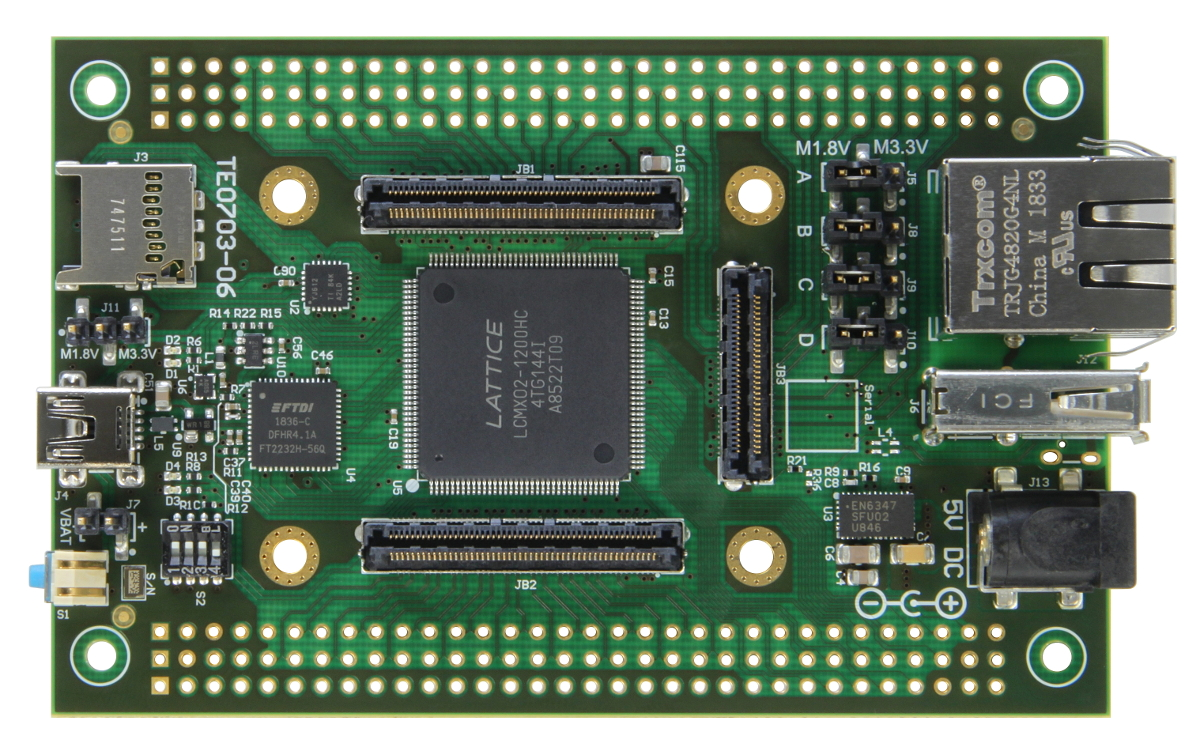
\includegraphics[scale=0.23]{imagenes/TE0703-06_1.jpg}
	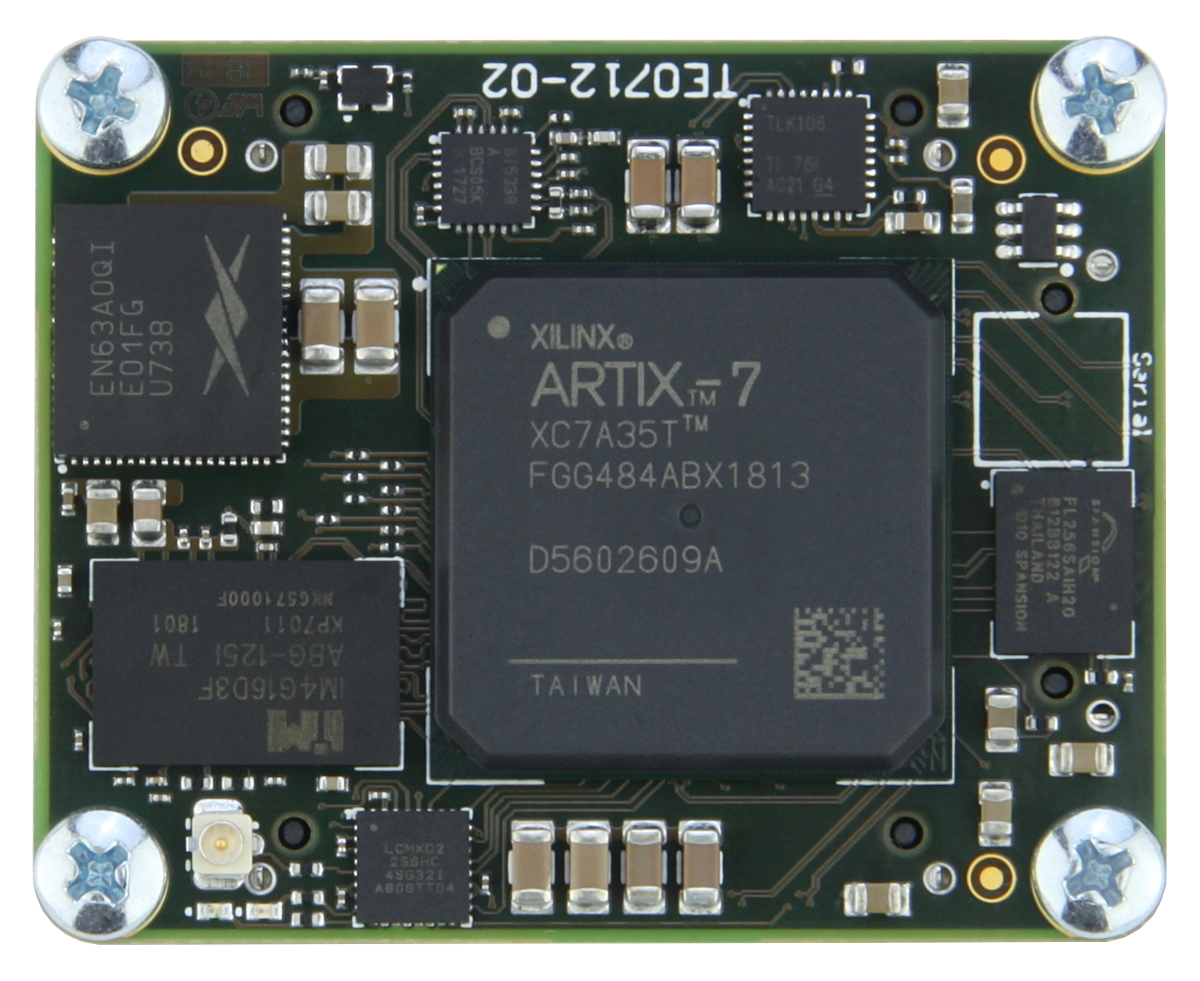
\includegraphics[scale=0.13]{imagenes/TE0712-02-35-2I_1.jpg}
	\caption{Placa de desarrollo y módulo FPGA a utilizar. A la izquierda se ilustra la placa de desarrollo Trenz TR0703\cite{TrenzElectronic2019TR0703Wiki} y a su derecha se ilustra el módulo que va montado en ella: Trenz TR0712\cite{TrenzElectronic2019TR07012Wiki} que contiene una FPGA Artix 7\cite{Xilinx20107DS180}.}
	\label{fig:trenz}
\end{figure}


Para esta alternativa de solución se consideran 32 canales de entrada LVDS ya que en el futuro será necesario conectar al menos 2 detectores de 16 canales en una misma FPGA. Para este proyecto en particular se probará el sistema con un solo detector de muones, por lo que la prueba e integración de un segundo detector queda pendiente y no se implementará en esta etapa. La figura \ref{fig:ministgc} ilustra los canales que posee un solo detector de muones de $15cm^2$.

\begin{figure}[H]
	\centering
	\includegraphics[scale=0.5]{imagenes/ministgc.pdf}
	\caption{Esquema de los canales provenientes de un detector Mini sTGC. Posee 8 tiras adyacentes de 15cm de largo por 1cm de ancho para cada eje coordenado. Cada tira emitirá un pulso analógico si una partícula cargada pasa través de ella. Se emitirán también pulsos de menor amplitud para el caso en que la partícula pase por una tira adyacente del mismo eje coordenado dentro de un radio específico. Este detector se posiciona perpendicularmente respecto a la fuente de radiación y en paralelo a (por debajo o por sobre) el sistema de disparo que indicará si la partícula captada corresponde o no a un muón. }
	\label{fig:ministgc}
\end{figure}

Las señales generadas por un detector son adaptadas por una tarjeta de interfaz ASD\cite{1999ATLASICs}, ilustrada en la figura \ref{fig:asd}. Esta tarjeta es capaz de capturar 16 señales simultaneas, por lo que es hardware suficiente para captar las señales de ambos ejes de un solo detector de muones.

\begin{figure}[H]
	\centering
	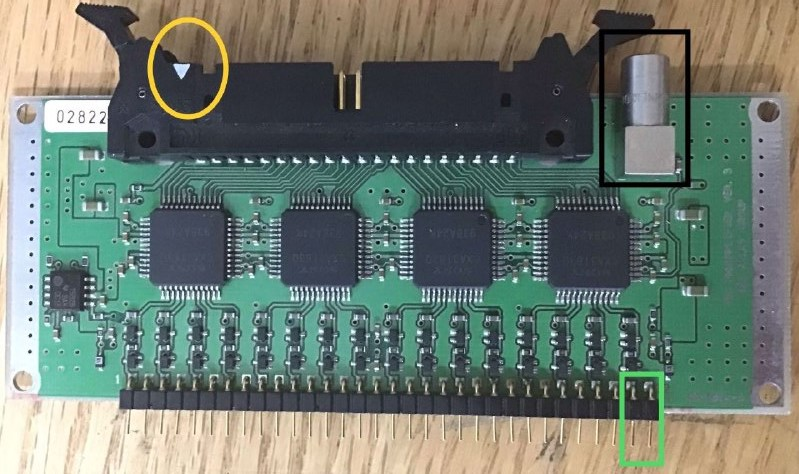
\includegraphics[scale=0.4]{imagenes/asd.jpg}
	\caption{Placa ASD\cite{1999ATLASICs} (Amplificator Shaper Discriminator), encargada de captar los 16 pulsos provenientes de un detector y entregar pulsos digitales asociados a ellos en su salida. El detector se conecta en sus entradas DIP ubicadas en su extremo inferior, mientras que las señales LVDS de salida se ubican en el conector de 40 puertos para cable plano en su extremo superior.}
	\label{fig:asd}
\end{figure}

\begin{figure}[H]
	\centering
	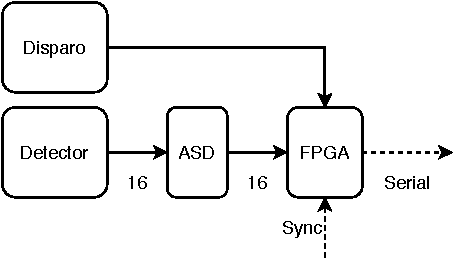
\includegraphics[scale=0.75]{imagenes/fpga1.pdf}
	\caption{Diagrama de bloques utilizando una FPGA como alternativa de solución. Se indica una salida serial para transmitir los resultados del análisis básico a algún procesador o memoria de alguna etapa posterior. La señal de sincronización ``Sync'' tiene como objetivo sincronizar la recolección y procesamiento de eventos, para que estos sean consistentes entre detectores.}
	\label{fig:fpga1}
\end{figure}


La idea en esta alternativa de solución es guardar los pulsos provenientes de la placa ASD en memoria temporal hasta la llegada de una señal de disparo. Un módulo que maneja la memoria será el encargado de tomar los pulsos correspondientes al disparo recibido y liberar la memoria de aquellos datos ya leídos u obsoletos, entregando la información útil a una siguiente etapa. Los pulsos aceptados serán entonces relacionados como parte de un mismo eventos y se estimará la duración de estos, generando y guardando así un arreglo de datos con identificador de pulso y duración. La última etapa se encargará de efectuar una operación capaz de determinar la posición del evento a partir de las duraciones medidas y los pulsos detectados, comunicando así un arreglo básico y preprocesado que incluya posición espacial y magnitud aproximada.


\begin{figure}[H]
	\centering
	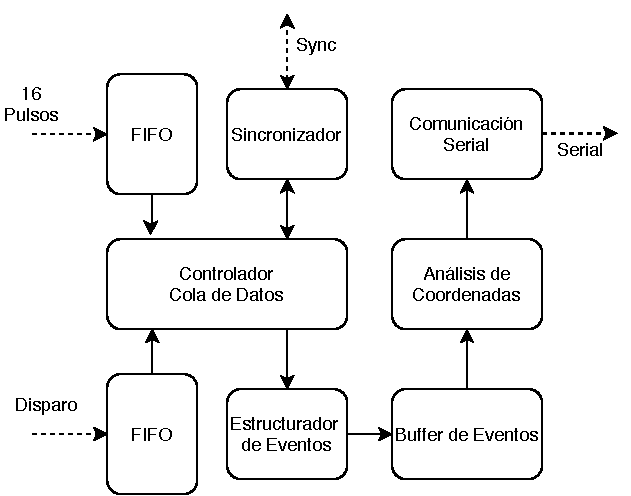
\includegraphics[scale=0.75]{imagenes/fpga2.pdf}
	\caption{Representación de la lógica interna de la FPGA. Se incluye una cola de datos para las señales de disparo, para los pulsos digitales provenientes de la ASD y una memoria de almacenamiento temporal para los eventos ya estructurados. Los bloques controlador, estructurador y análisis cumplen las funciones de aceptar o descartar pulsos, cuantificar anchos de pulso a  los canales asociados y determinar coordenada del cruce de un muón respectivamente.}
	\label{fig:fpga2}
\end{figure}

Se espera que para lograr el escalamiento se incluya una señal para mantener la lectura de eventos sincronizada entre distintas FPGA. Además, se deberá incluir un modulo de comunicación para entregar la información captada a una etapa posterior con un análisis más detallado, encargado de reunir todos los eventos de diferentes FPGAs.


%\newpage
%\section{Conclusión}
%\par Luego de presentar y evaluar diferentes alternativas de solución, el análisis indica que la mejor solución corresponde a implementar el sistema en una FPGA, obteniendo un resultado de 8.4 puntos según los criterios de selección. Esta alternativa fue precisamente la que se ha considerado desde un principio y coincide con ser la tecnología más utilizada dentro del desarrollo de sistemas de adquisición para física de partículas\cite{Basiladze2017Methods1}\cite{Basiladze2017Methods2}.
%\par Esta alternativa fue seleccionada por sobre las demás debido a su destacado desempeño, ya que cuenta con mayor frecuencia de reloj disponible, gran cantidad de recursos y suficientes puertos LVDS. Este último requerimiento es necesario para recibir los pulsos digitales capturados por la interfaz ASD provenientes del detector, los cuales se emiten bajo el estándar LVDS para transmisión de señales diferenciales.
%\par Destaca también esta alternativa al ser una plataforma flexible, en sentido de brindar las posibilidades de adaptar el diseño propuesto sin tener que adquirir nuevo equipamiento. Esta versatilidad es intrínseca de las FPGAs, las cuales se caracterizan por permitir un gran control en el diseño del hardware a bajo nivel.
%\par Luego de este trabajo de selección y detalle de la solución, ya se encuentran definidos los objetivos principales del proyecto y los esquemas generales del diseño a implementar para cumplir con ellos. Con la información presentada en la sección \ref{alternativa} es posible comenzar las etapas de planificación y posterior ejecución del proyecto, para desarrollar así un sistema de adquisición de datos para detectores de muones escalable basado en FPGA.

